%
% tracking.tex -- Verfolgen einer Sternposition und Kontrolle eines Teleskops
%
% (c) 2013 Prof Dr Andreas Mueller, Hochschule Rapperswil
%
\subsection{Nachf"uhrung und ihre Kalibrierung}
Wie verfolgt man ein Objekt mit einer Kamera?
Offenbar muss man dazu
die Bilder der Kamera analysieren, die Verschiebung des Objektes innerhalb
des Bildes feststellen, und die Halterung der Kamera so zu bewegen,
dass das Objekt erneut zentriert erscheint.
Damit dies m"oglich ist, muss man wissen, wie stark sich die Steuersignale
der Halterung auf die Verschiebung des Bildes in der Kamera auswirken.

In der Astronomie werden besonders hohe Anforderungen an die Pr"azision
einer solchen Steuerung gestellt, schliesslich will man da ein grosses
Teleskop w"ahrend Stunden auf den gleichen Punkt am Himmel richten, um
zum Beispiel eine Aufnahme einer Galaxie entsprechend lange belichten
zu k"onnen.
Dabei darf die Abweichung nie gr"osser als Bruchteile eines
einer Winkelsekunde werden, da sonst das Bild unscharf w"urde.

Astronomische Teleskop werden daher oft auf einer sogenannten
"aquatorialen Montierung eingesetzt, welche eine Achse parallel
zur Erdeachse hat. Dreht man diese Achse mit genau der gleichen
Geschwindigkeit wie die Erde, aber in entgegengesetzter Richtung,
sollte sich die Drehung aufheben. In der Praxis verbleibt durch
Aufstellungsfehler und Atmosph"areneinfl"usse trotzdem ein Restfehler,
der gemessen und korrigiert werden muss.

\subsubsection{Guiding}
Nachf"uhrung oder Guiding beschreibt den Prozess, durch geeignete
Korrektursignale an die Montierung des Teleskops, ein Objekt, meist
einen einzelnen, leicht zu identifizerenden Stern, st"andig an der
gleichen Stelle auf dem CCD-Chip der Kamera zu halten. Dazu wird
eine Hilfskamera-verwendet, die entweder mit einem eigenen kleinen
Teleskop, dem Leitfernrohr, ausgestattet ist, oder die das Licht
des Sterns aus dem Strahlengang des Hauptteleskops erh"alt, wo
es mit Hilfe eines kleine Spiegels auf den CCD-Chip der Nachf"uhrkamera
ausgelenkt wird.

Die Montierung kann typischerweise in zwei senkrechten Richtungen
bewegt werden, zus"atzlich zu der konstanten Drehung um die
Achse parallel zur Erdachse.
Wir nehmen an, dass wir die Geschwindigkeit
dieser zus"atzlichen Bewegung im Interval $[-1,1]$ angeben k"onnen.
In der Praxis kann man jedoch meistens die Extremgeschwindigkeiten
$\pm 1$ aktivieren. Um die mittlere Geschwindigkeit $0.2$ zu erhalten,
muss man also die Geschwindigkeit $+1$ w"ahrend 200ms aktivieren.

Bei einer "aquatorialen Montierung entsprechen die Bewegungsrichtungen,
die man mit diesen Steuersignalen erreichen kann, der geographischen
L"ange und Breite auf der Himmelskugel. Die Astronomen kennen diese
Koordinaten als Rektaszension, die Bewegung um die Erdachse, und Deklination,
sie verwenden meist $\alpha$ und $\delta$ f"ur die beiden Winkel.

Es ist klar, dass eine Bewegung in Deklination immer die gleiche Auswirkung
auf ein Sternbild in der Kamera hat.
Die Auswirkung einer Bewegung um Erdachse h"angt jedoch
davon ab, ob ein Objekt nahe des "Aquators oder nahe des Pols
betrachtet wird. Wird das Teleskop parallel zur Erdachse ausgereichtet
($\delta=90^\circ$), dann bewegt sich ein Stern im Zentrum des Bildfeldes
bei Drehung um die Erdachse "uberhaupt nicht.
Je nach Position des Objektes auf der Himmelskugel sind also andere
Korrektursignale erforderlich, um das Objekt im Zentrum des CCD-Chips
zu halten.

Die Hilfskamera liefert Bilder des Leitsterns, aus denen die genaue
Position des Sternes im Koordinatensystem des CCD-Chips gemessen
werden kann. Die Achsen dieses Koordinatensystems m"ussen dabei
"uberhaupt nichts mit den Richtungen f"ur Rektaszension und Deklination
zu tun haben.

\subsubsection{Kalibrierung}
Ohne irgendwelche Korrektursignale wird der Leitstern ungef"ahr mit
gleichf"ormiger Geschwindigkeit $v$ "uber den CCD-Chip driften.
Wendet man Korrektursignale $(\alpha,\delta)$ an, kommt eine
weitere Bewegung hinzu. F"ur die Regelung brauchen wir den Zusammenhang
zwischen $(\alpha,\delta)$ und der zugeh"origen Verschiebung $(x,y)$ auf dem
CCD-Chip. Der Zusammenhang muss linear sein:
\begin{equation}
\begin{linsys}{3}
x&=&a_{11}\alpha&+&a_{12}\delta&+&tv_1\\
y&=&a_{21}\alpha&+&a_{22}\delta&+&tv_2\\
\end{linsys}
\qquad
\Leftrightarrow
\qquad
\begin{pmatrix}x\\y\end{pmatrix}
=A\begin{pmatrix}\alpha\\\delta\end{pmatrix}+tv
\label{guiding:model}
\end{equation}
Wir m"ussen die Matrix $A$ und den Vektor $v$ ermitteln.

Um Daten f"ur die Bestimmung von $A$ und $v$ zu bekommen, kann man wie
folgt vorgehen. Man f"ahrt mit dem Teleskop nacheinander alle Gitterpunkte
eines $2\times 2$ Quadrates mit den Ecken
$(-1,-1)$ und $(1,1)$ im $(\alpha,\delta)$-Koodinatensystem an.
\begin{figure}
\begin{center}
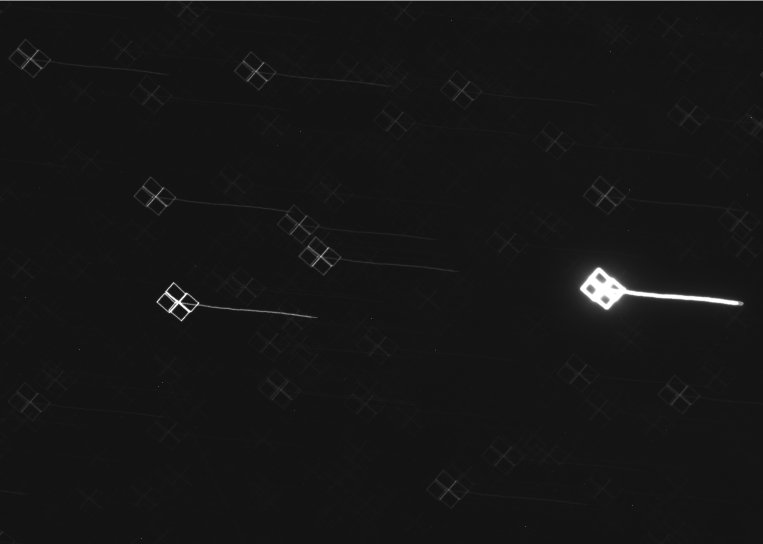
\includegraphics[width=\hsize]{graphics/calibration.jpg}
\end{center}
\caption{Bewegung des Leitsterns w"ahrend des Kalibrierungsprozesses
und dem anschliessenden Anfahren der Nachf"uhrposition,
Langzeitaufnahme mit der Hauptkamera.
Gut zu erkennen ist auch, dass nicht ein Quadrat entsteht. Das Bild
entstand bei der Kalibrierung f"ur die Aufnahmen, aus denen 
Abbildung~\ref{andromeda-image} zusammengesetzt ist, also bei
einer Deklination von ca.~$40^\circ$.
\label{guiding:calibration}}
\end{figure}
Abbildung \ref{guiding:calibration} zeigt eine Langzeitbelichtung der
Hauptkamera w"ahrend des Kalibrierungsprozesses.
Nach jeder Bewegung misst man die Position des Leitsterns neu, und
notiert auch die Zeit. F"ur jede Position $(\alpha_i,\delta_i)$
bekommt man eine Zeit $t_i$ und eine Leitstern-Position $(x_i,y_i)$.
Wenn die Transformation (\ref{guiding:model}) zutrifft, m"ussten die
beiden Gleichungen
\[
\begin{linsys}{6}
x_i&=&\alpha_ia_{11}&+&\delta_ia_{12}&+&t_iv_1& &              & &              & &      \\
y_i&=&              & &              & &      & &\alpha_ia_{21}&+&\delta_ia_{22}&+&t_iv_2\\
\end{linsys}
\]
erf"ullt sein. F"ur die $n=9$ Positionen des Quadrates ergibt dies insgesamt
$2n=18$  Gleichungen f"ur die sechs Unbekannten $A$ und $v$.
Das Gleichungssystem ist zwar "uberbestimmt, 
es l"asst sich aber mit der Methode von Abschnitt \ref{section:ueberbestimmt}
effizient l"osen. 

\subsubsection{Korrektur}
Wir jetzt eine Positions-Abweichung $(x,y)$ des Leitsterns gemessen,
kann aus $A$ und $v$ die Korrektur in Rektaszension und Deklination
ermittelt werden, mit der die Abweichung innert $t=1$ Sekunde wieder
zum Verschwinden gebracht werden kann. Dazu muss man nur
(\ref{guiding:model}) nach $(\alpha,\delta)$ aufl"osen:
\[
\begin{pmatrix}x\\y\end{pmatrix}
=
A\begin{pmatrix}\alpha\\\delta\end{pmatrix}+tv
\qquad
\Rightarrow
\qquad
\begin{pmatrix}\alpha\\\delta\end{pmatrix}=
A^{-1}\left(
\begin{pmatrix}
x\\y
\end{pmatrix}
-tv
\right).
\]
Die Kalibrationsdaten $A$ und $v$ h"angen offenbar nur von der relativen
Orientierung der Leitkamera zu den Achsen des Himmelskoordinatensystems
ab, sowie von der Deklination des Zielobjektes.
Insbesondere muss die
Kalibration nur einmal durchgef"uhrt werden, solange man nur Objekte verfolgen
will, deren Deklination nicht sehr verschieden ist, und die Leitkamera in ihrer
Fassung nicht gedreht wird.

\subsubsection{Qualit"atsbeurteilung der Kalibration}
Wie erkennt man, ob die Kalibrationsdaten eine erfolgreiche Nachf"uhrung
erm"oglichen werden. Montierungsunzul"anglichkeiten wie "uberm"assig 
viel Spiel des Antriebs k"onnte dem entgegenstehen.

Auf einer perfekten Montierung wird sich der Leitstern w"ahrend er 
Kalibrierung exakt entlang des Gitters bewegen. Die beiden Spaltenvektoren
\[
a_1=\begin{pmatrix}a_{11}\\ a_{21}\end{pmatrix}
\quad\text{und}
\quad
a_2=\begin{pmatrix}a_{12}\\ a_{22}\end{pmatrix}
\]
sollten also senkrecht stehen. Dies ist sehr einfach zu pr"ufen:
das Produkt $AA^t$ sollte eine Diagonalmatrix sein. Die Gr"osse der
Ausserdiagonalelement der Matrix $AA^t$ gibt also an, wie gut die Kalibrierung
gelungen ist.
Als dimensionslose  Masszahl f"ur die Kalibrierungsqualit"at
eignet sich der Quotient
\[
\frac{a_1\cdot a_2}{\det(A)}.
\]
Werte nahe bei $0$ deuten auf eine gute Kalibrierung hin.
